
\documentclass[11pt]{beamer}
\usepackage{helvet} %font
\beamertemplatenavigationsymbolsempty
\usetheme{JuanLesPins}
\usefonttheme{structurebold}

\usepackage[french]{babel}
\usepackage[utf8]{inputenc}
\usepackage[T1]{fontenc}
\usepackage{amssymb,amsmath}
\usepackage{tikz}
\usepackage{geometry}
\usepackage{xcolor,colortbl}
\usetikzlibrary{arrows,positioning}
\usepackage{listings}

\AtBeginSubsection[]
{
   \begin{frame}
	\small \tableofcontents[currentsection]
   \end{frame}
}

\newenvironment{slide}[1]{%
\begin{frame}[environment=slide]
\frametitle{#1}
}{%
\end{frame}
}
\setbeamercolor{structure}{fg=red}
\setbeamercolor{frametitle}{bg=black,fg=white}
\definecolor{gris}{gray}{0.6}
\definecolor{grisclair}{gray}{0.9}

\newtheorem{exercice}{Exercice}

\title{Machine Learning II \\ Introduction à \texttt{matplotlib}}
\author{Nicolas Bourgeois}
\date{}

\newcommand{\Python}[1]{
	{\small	\lstinputlisting[language=Python]{./#1.py}}
}
\newenvironment{pyenvsmall}
	{ \ttfamily \tiny }
	{\par  }

\newcommand{\Pythonsmall}[1]{
	{\scriptsize \lstinputlisting[language=Python]{./#1.py}}
}
\newcommand{\elimine}[1]{{\textcolor{lightgray}{#1}}}

\newcommand\Wider[2][3em]{%
\makebox[\linewidth][c]{%
  \begin{minipage}{\dimexpr\textwidth+#1\relax}
  \raggedright#2
  \end{minipage}%
  }%
}

\begin{document}

\begin{frame}
\maketitle
\end{frame}

\begin{frame}{Télécharger}

Data and Cheatsheets :\\
\vspace{0.3cm}

\url{ouralou.fr/Resources/epita/C2.zip}


\end{frame}


\begin{frame}{Exercice}
\begin{exercice}
Affichez les fonctions $x \mapsto e^{-\lambda x}$ pour diverses valeurs du paramètre $\lambda$. N'oubliez pas l'axe et la légende.
\end{exercice}

\begin{exercice}
Même question, mais les courbes doivent être sur des sous-figures différentes et non superposées.
\end{exercice}
\end{frame}

\begin{frame}{Résultat attendu (1)}
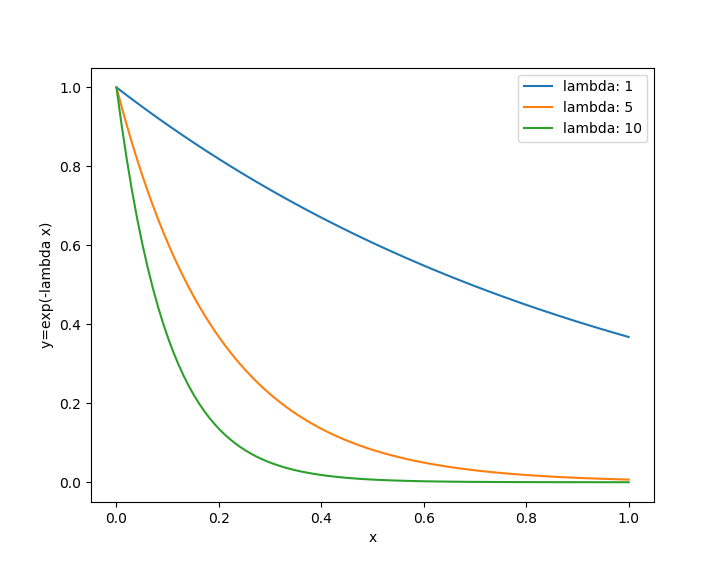
\includegraphics[scale=0.45]{ex201}
\end{frame}

\begin{frame}{Résultat attendu (2)}
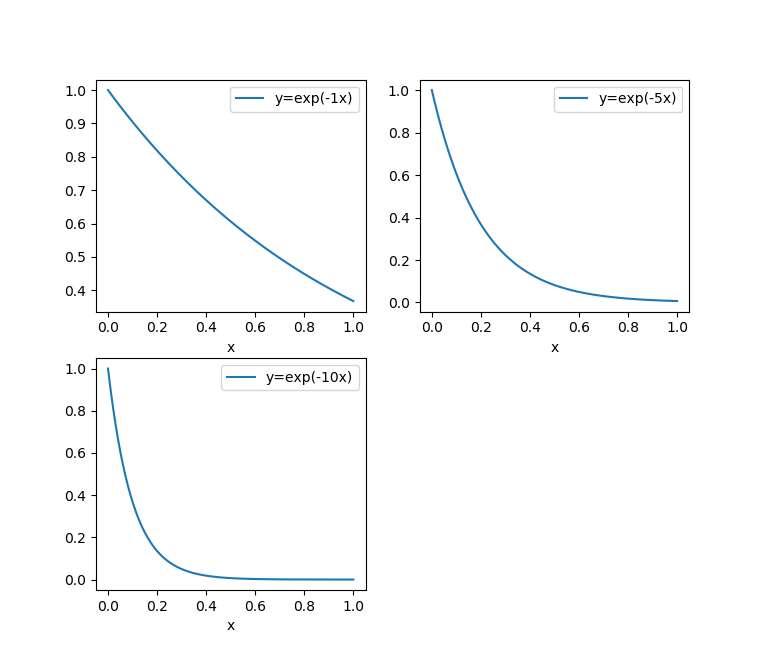
\includegraphics[scale=0.45]{ex202}
\end{frame}

\begin{frame}{Solution - Première partie}
\Python{ex201}
\end{frame}

\begin{frame}{Solution -Deuxième partie}
\Python{ex202}
\end{frame}

\begin{frame}{Exercice}
\begin{exercice}
Reprenez les courbes du premier exercice et annotez-les pour distinguer les points $y=e^{-1}$.
\end{exercice}
\end{frame}

\begin{frame}{Résultat attendu}
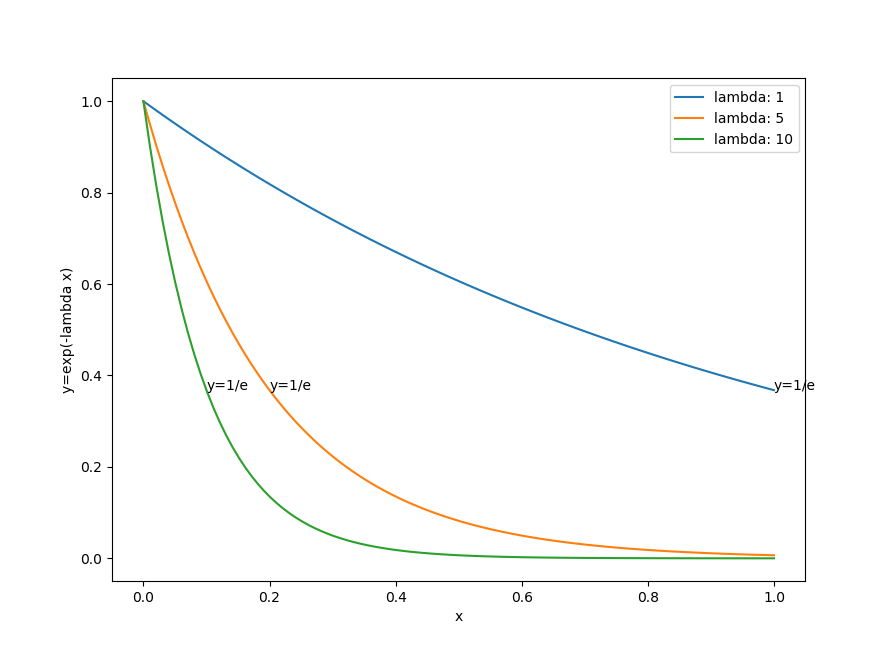
\includegraphics[scale=0.45]{ex203}
\end{frame}

\begin{frame}{Solution}
\Python{ex203}
\end{frame}

\begin{frame}{Exercice}
\begin{exercice}
Importez les données de data1.csv dans un dataframe et affichez leur dispersion selon les axes age et prix du billet.
\end{exercice}
\begin{exercice}
Modifiez la couleur et ajoutez une légende de façon à faire apparaître l'information si la personne a survécu ou non.
\end{exercice}
\end{frame}

\begin{frame}{Résultat attendu (1)}
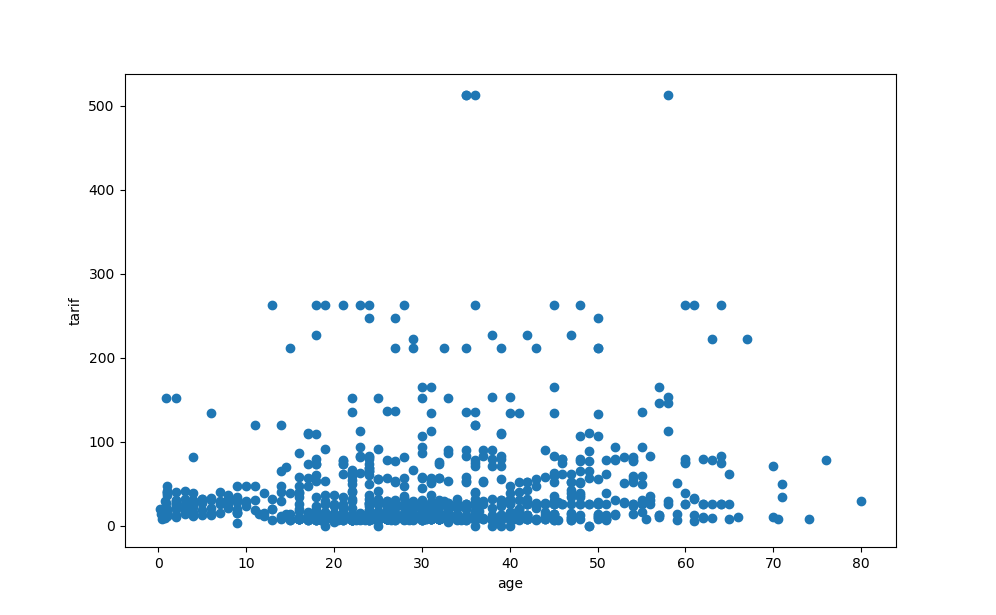
\includegraphics[scale=0.45]{ex203bis}
\end{frame}

\begin{frame}{Résultat attendu (2)}
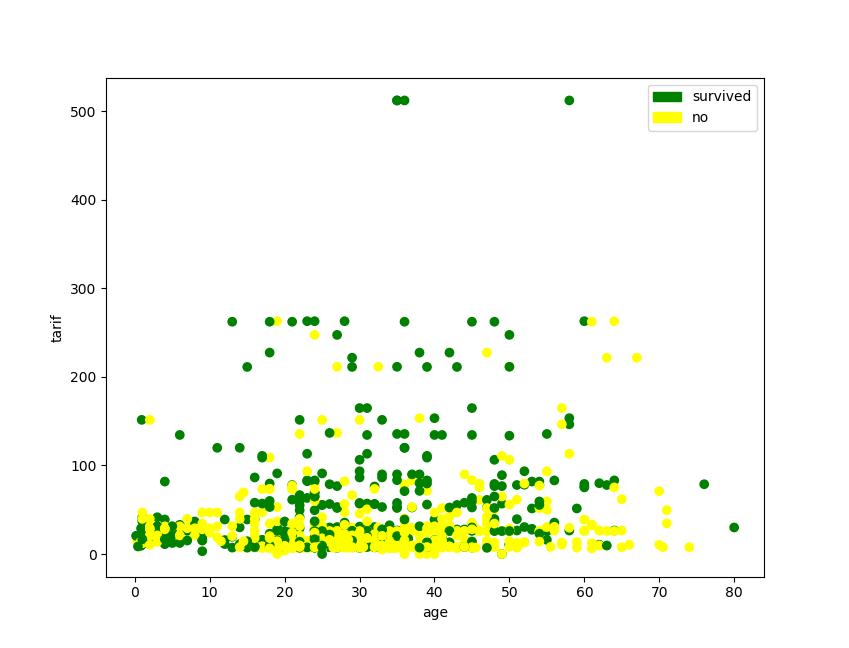
\includegraphics[scale=0.45]{ex204}
\end{frame}

\begin{frame}{Solution - première partie}
\Python{ex203bis}
\end{frame}

\begin{frame}{Solution - deuxième partie}
\Python{ex204}
\end{frame}

\begin{frame}{Exercice}
\begin{exercice}
Utilisez une scatter matrix pour croiser les données age et prix du billet, tout en gardant la couleur pour évaluer la survie.
\end{exercice}
\begin{exercice}
Ajoutez le genre pour rendre la scatter matrix utile. Vous devrez convertir le type de données.
\end{exercice}
\begin{exercice}
Ajoutez un facteur de dispersion aléatoire des points autour de la valeur genre de façon à mieux les visualiser.
\end{exercice}
\end{frame}

\begin{frame}{Résultat attendu (1)}
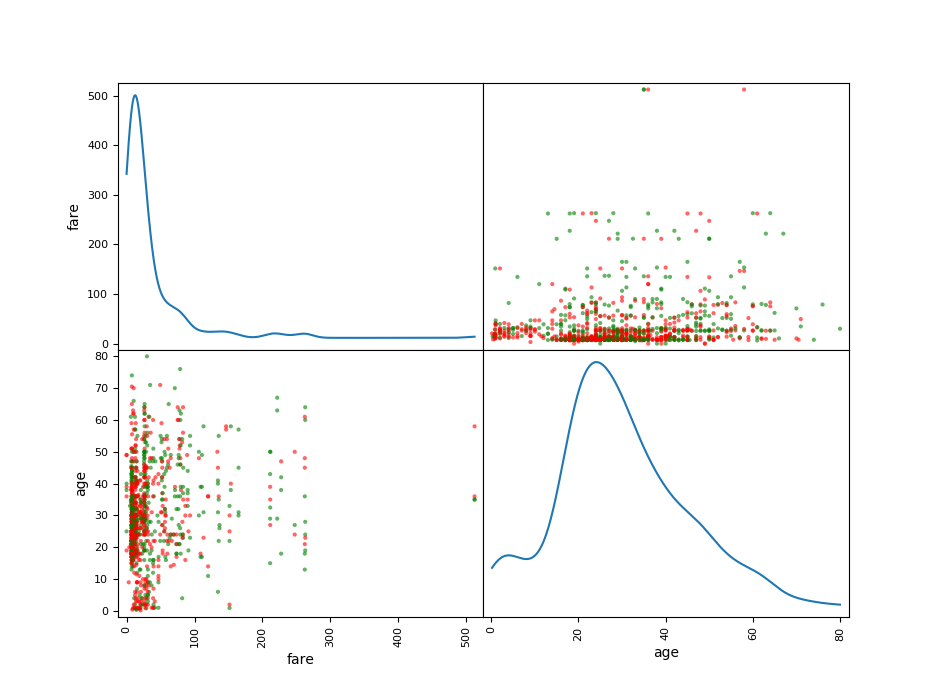
\includegraphics[scale=0.42]{ex205}
\end{frame}

\begin{frame}{Résultat attendu (2)}
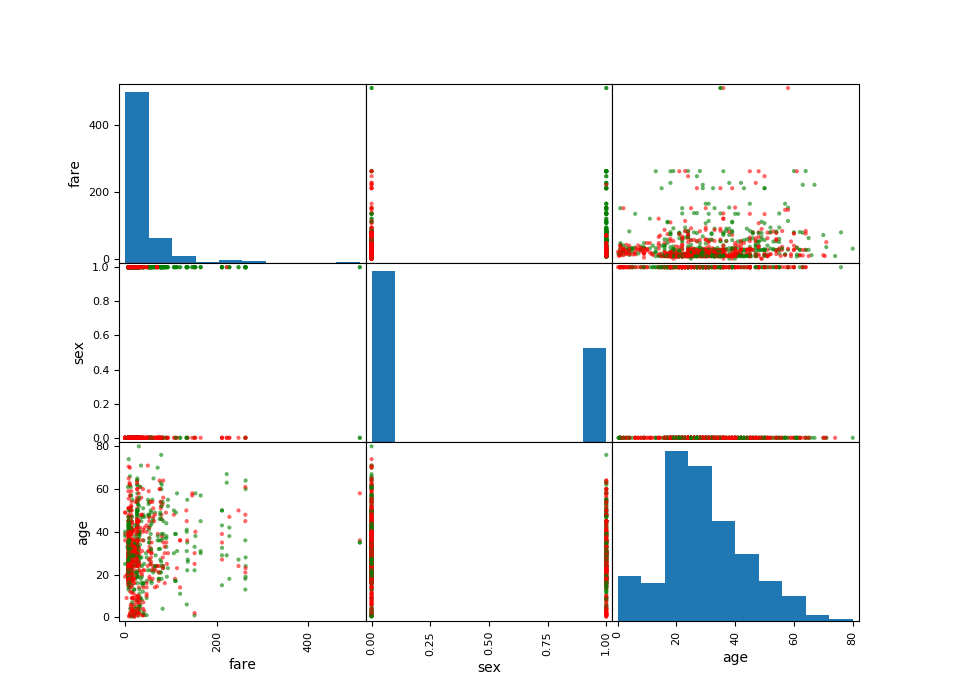
\includegraphics[scale=0.42]{ex206}
\end{frame}

\begin{frame}{Résultat attendu (3)}
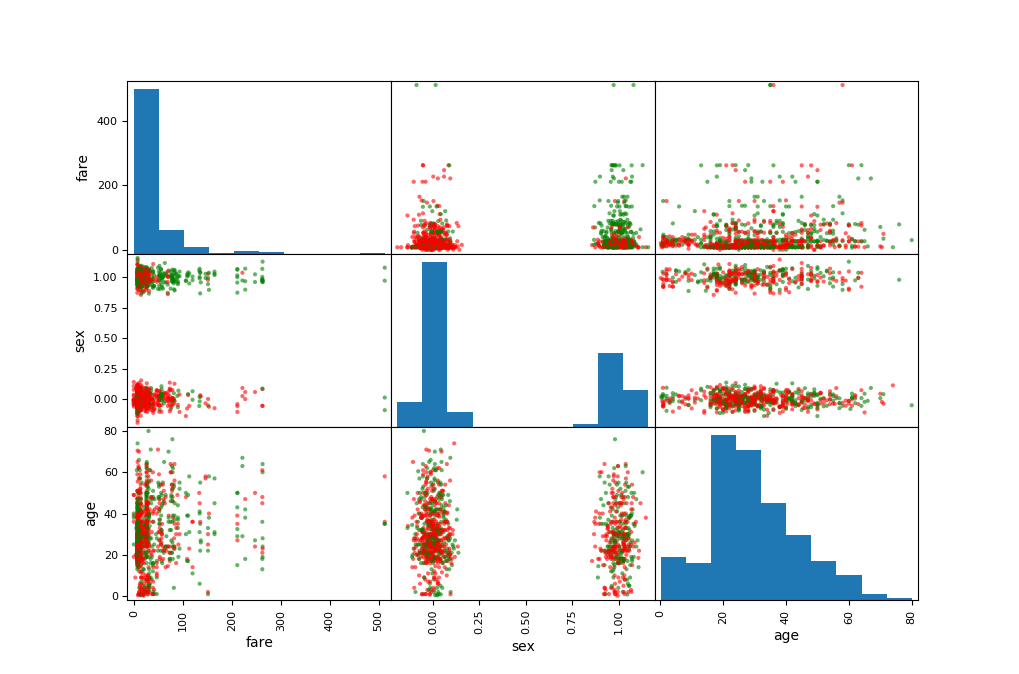
\includegraphics[scale=0.42]{ex207}
\end{frame}

\begin{frame}{Solution - première partie}
\Wider{\Python{ex205}}
\end{frame}

\begin{frame}{Solution - deuxième partie}
\Wider{\Python{ex206}}
\end{frame}

\begin{frame}{Solution - troisième partie}
\Wider{\Python{ex207}}
\end{frame}


\end{document}